\documentclass{report}
\usepackage[margin=1in, paperwidth=8.5in, paperheight=11in]{geometry}
%Math packages%
\usepackage{amsmath}
\usepackage{amsthm}
%Spacing%
\usepackage{setspace}
\onehalfspacing
%Lecture number%
\newcommand{\lectureNum}{4}
%Variables - Date and Course%
\newcommand{\curDate}{February 1, 2017}
\newcommand{\course}{MATH 239}
\newcommand{\instructor}{}
%Defining the example tag%
%\theoremstyle{definition}%
\newtheorem{ex}{Example}[section]
%Setting counter given the lecture number%
\setcounter{chapter}{\lectureNum{}}
%Package for drawing graphs%
\usepackage{tikz}
\usepackage{verbatim}
\usetikzlibrary{arrows}

\begin{document}
%Note title%
\begin{center}
\begin{Large}
\textsc{\course{} | Tutorial \lectureNum{}}
\end{Large}
\end{center} 
\noindent \textit{Bartosz Antczak} \hfill
\textit{\curDate{}}
\rule{\textwidth}{0.4pt}
% Actual Notes%
\section*{Problem 1 | Building an MST}
Given the weighted graph
\begin{center}
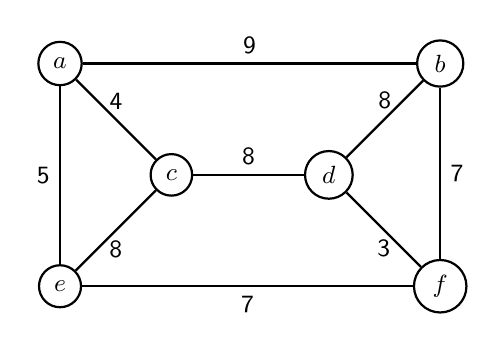
\begin{tikzpicture}[-,auto,node distance=2cm,
                    thick,main node/.style={circle,draw,font=\sffamily\small}]

  \node[main node] (1) {$c$};
  \node[main node] (2) [above left of=1] {$a$};
  \node[main node] (3) [below left of=1] {$e$};
  \node[main node] (4) [right of=1] {$d$};
  \node[main node] (5) [below right of=4] {$f$};
  \node[main node] (6) [above right of=4] {$b$};
  
  \path[every node/.style={font=\sffamily\small}]
    (1) edge node [above] {4} (2)
    	edge node [below] {8} (3)
    	edge node [above] {8} (4)
    (2) edge node [left] {5} (3)
    	edge node [above] {9} (6)
    (4) edge node [above] {8} (6)
    	edge node [below] {3} (5)
    (5) edge node [below] {7} (3)
    	edge node [right] {7} (6);
\end{tikzpicture}
\end{center}
%TODO draw graph 1%
Construct an MST.
\begin{center}
\begin{tabular}{ c c c }
Iteration & Edge added & Vertex Added \\
0 & | & $b$ \\
1 & $bf$ & $f$ \\
2 & $df$ & $d$ \\
3 & $ef$ & $e$ \\
4 & $ae$ & $a$ \\
5 & $ac$ & $c$ \\
\end{tabular}
\end{center}
The tree $T$, where $E(T) = \{bf, df, ef, ae, ac\}$, is an MST, by Prim's algorithm.
\section*{Problem 2 | Proving a Statement}
Prove that if $G$ is 3-regular and bipartite, it cannot  have a bridge.
\subsubsection{Proof:}
Suppose not. Then $G$ has a bridge $e = uv$, $e \in E(G)$. Let $K$ be the component of $G-e$ that contains $u$. Since $G$ is bipartite, then $K$ is bipartite. Also, $K$ is nearly 3-regular, except for $u$, which is 2-regular (since we deleted one of its edges).\\
Consider the bipartition of $K$, call them $A$ and $B$. Since $u \in K$, $u$ is in one of the bipartitions, let's put it in $A$. Observe that the number of edges in $A$ is the same as in $B$ (by definition of a bipartition). In $A$, there are $3(\vert A \vert - 1) + 2$ edges, and in $B$, there are $3\vert B \vert$ edges. However, the number of edges in $A$ is not divisible by 3 but the number of edges in $B$ are. This means that both partitions have a different number of edges | a contradiction. Therefore, $G$ cannot have a bridge.
%END%

\end{document}